\documentclass{article}

% if you need to pass options to natbib, use, e.g.:
%     \PassOptionsToPackage{numbers, compress}{natbib}
% before loading neurips_2026

% ready for submission
\usepackage{neurips_2026}

\usepackage[utf8]{inputenc} % allow utf-8 input
\usepackage[T1]{fontenc}    % use 8-bit T1 fonts
\usepackage[colorlinks=true, citecolor=blue, linkcolor=blue, urlcolor=blue]{hyperref}       % hyperlinks
\usepackage{url}            % simple URL typesetting
\usepackage{booktabs}       % professional-quality tables
\usepackage{amsfonts}       % blackboard math symbols
\usepackage{nicefrac}       % compact symbols for 1/2, etc.
\usepackage{microtype}      % microtypography
\usepackage{xcolor}         % colors
\usepackage{amsmath, amssymb, amsthm}
\usepackage{graphicx}
\usepackage{algorithm}
\usepackage{algorithmic}

\title{Cheap Talk is Expensive: Quantifying the Strategic Value of Language in Imperfect Information Games}

\author{%
  Anonymous Authors \\
  Affiliation \\
  \texttt{email@domain.com} \\
}

\date{}

\begin{document}


\maketitle

\begin{abstract}
While AI has achieved superhuman mastery in mathematical strategy games like Poker, it remains a "mute savant," fundamentally incapable of the psychological dimension of natural language interaction (Cheap Talk). Existing neuro-symbolic approaches either focus on cooperative dialogue (e.g., Cicero) or pure regret minimization, leaving adversarial belief manipulation in zero-sum settings unsolved. In this work, we introduce \textbf{Talk-CFR}, the first framework to integrate a Strategic Module (Deep CFR) with a Linguistic Module (LLM) by treating natural language as a discrete, strategic action within the game tree. We propose a novel metric, \emph{Linguistic Value (LV)}, to quantify the chip-value of speech. We observe an emergent deceptive mixing regime in which the agent strategically calibrates truthful vs. fabricated statements to influence opponent beliefs while avoiding predictability, providing empirical evidence that cheap-talk can have measurable strategic value precisely when opponents exhibit systematic miscalibration in belief updating.
\end{abstract}

\section{Introduction}
The intersection of Game Theory and Artificial Intelligence has witnessed monumental strides in recent years. Algorithms such as DeepStack \citep{moravcik2017deepstack} and Libratus \citep{brown2018superhuman} have achieved superhuman mastery in imperfect information games like Heads-Up No-Limit Texas Hold'em. By leveraging Counterfactual Regret Minimization (CFR) and its deep learning variants \citep{brown2019deep}, these agents can navigate vast game trees and resolve uncertainty with mathematical precision. However, despite their tactical brilliance, these agents remain "mute savants." They play in silence, treating the game purely as a sequence of mechanical actions (bet, check, fold), ignoring a fundamental dimension of real-world strategic interaction: \textit{communication}.

In human poker, negotiation, and geopolitical maneuvers, speech is not merely decorative; it is a strategic instrument. This phenomenon, known in economic theory as "Cheap Talk" \citep{crawford1982strategic}, refers to costless, non-binding communication that can nonetheless influence the outcomes of a game by altering the belief states of opponents. A player might feign confidence to bluff a weak hand or downplay a strong one to induce a bet. Existing neuro-symbolic approaches, such as Cicero \citep{bakhtin2022mastering}, have successfully integrated Large Language Models (LLMs) with planning algorithms, but they have primarily focused on \textit{cooperative} settings like Diplomacy, where honest communication is incentivized to form alliances. The challenge of \textit{adversarial} communication in zero-sum games—where deception is not just an option but a necessity for optimal play—remains largely unexplored in the Deep Reinforcement Learning (DRL) landscape.

In this work, we introduce \textbf{Talk-CFR}, a novel framework that bridges the gap between the mathematical rigor of CFR and the linguistic expressivity of LLMs. We conceptualize natural language not as external noise, but as a discrete, strategic action within the game tree itself. Our "Dual-Brain" architecture consists of a \textbf{Strategist} (a Deep CFR agent) that computes the optimal strategic intent (e.g., "Induce Fold" or "Value Bet"), and a \textbf{Speaker} (a fine-tuned LLM) that translates this intent into contextually appropriate natural language utterances.

Our contributions are threefold:
\begin{enumerate}
    \item \textbf{Formalization of Strategized Cheap Talk}: We formalize talk-augmented zero-sum imperfect-information games with an explicit public cheap-talk channel and clarify when babbling equilibrium should hold versus when Talk-CFR can exploit bounded rationality.
    \item \textbf{Intent-Level Abstraction}: We propose an intent-level abstraction that makes CFR tractable in the presence of an open-ended language channel, with LLMs used only for message realization, analyzing the trade-off between expressivity and abstraction error.
    \item \textbf{Linguistic Value (LV) Decomposition}: We introduce and validate LV as a measurable marginal value of communication, and empirically characterize when LV becomes positive under boundedly rational belief updates (e.g., distinguishing rational silence from effective "jamming").
\end{enumerate}

\section{Related Work}

\paragraph{Solving Imperfect Information Games}
The resolution of large-scale imperfect information games has historically relied on abstraction and iterative equilibrium finding. \citet{zinkevich2007regret} introduced CFR, which minimizes regret independently at each information set to converge to a Nash Equilibrium. This was scaled significantly by \citet{moravcik2017deepstack} and \citet{brown2018superhuman} using depth-limited subgame solving and neural function approximation (Deep CFR \citep{brown2019deep}). However, these methods operate in a "silent" mode, where the action space is restricted to game mechanics. Our work extends this paradigm by augmenting the action space with a communicative channel, requiring the solver to reason about the information leakage inherent in speech.

\paragraph{Language and Reinforcement Learning}
The integration of language into RL agents has gained traction with the advent of Transformers \citep{vaswani2017attention, sutskever2014sequence}. \citet{lewis2017deal} explored end-to-end learning of negotiation dialogues, where agents learned to haggle over items. More recently, \citet{bakhtin2022mastering} presented Cicero, an agent that achieved human-level performance in Diplomacy by combining a strategic planning module with a dialogue model. While Cicero is a landmark achievement, its success relies on the cooperative structure of Diplomacy, where "honesty is essentially the best policy" for maintaining long-term alliances. In contrast, our work focuses on the zero-sum domain \citep{foerster2016learning}, where interests are strictly opposed, and communication is fundamentally adversarial.

\paragraph{Emergent AI Agent Architectures}
The rapid evolution of LLM-based autonomous agents \citep{xi2023rise, wang2023survey, mialon2023augmented} has introduced new paradigms for problem-solving. Frameworks like Voyager \citep{wang2023voyager} and AutoGen \citep{wu2023autogen} demonstrate how agents can self-improve and collaborate. Recent works on "Generative Agents" \citep{park2023generative} and "Camel" \citep{li2023camel} explore social simulation, while Tree of Thoughts \citep{yao2024tree} and Reflexion \citep{shinn2023reflexion} enhance reasoning. Specialized multi-agent frameworks like MetaGPT \citep{hong2023metagpt} and Communicative Agents \citep{qian2023communicative} drive software development. Benchmarks such as AgentBench \citep{liu2023agentbench} and AlfWorld \citep{shridhar2020alfworld} provide rigorous evaluation grounds. However, as agents become more capable \citep{openai2023gpt4, team2023gemini, touvron2023llama}, the risk of "Deceptive Alignment" \citep{hubinger2019risks, sharma2023understanding} increases. Our work directly probes this risk, alignment with concerns in safety literature \citep{kenton2021alignment, anthropic2022constitutional}.

\paragraph{Signaling Games in Economics}
Our theoretical grounding draws from the literature on Signaling Games. \citet{crawford1982strategic} formalized "Cheap Talk," showing that informative communication is only possible when there is some alignment of interests. In zero-sum games, theory predicts that all talk should be ignored (the "Babbling Equilibrium"). However, psychological game theory suggests that humans are not perfectly rational Bayesian updaters; they are susceptible to framing and emotional manipulation. We hypothesize, and empirically verify, that against boundedly rational opponents (or opponents with imperfect belief models), cheap talk retains significant strategic value.

\paragraph{Neuro-Symbolic Game AI}
The convergence of connectionist learning and symbolic reasoning has emerged as a powerful paradigm for complex reasoning tasks. In game AI, this is often manifested as combining neural policy approximation with symbolic search (e.g., MCTS in AlphaGo). Our work proposes a different axis of neuro-symbolic integration: the \textit{Semiotic-Strategic} axis. Here, the "symbolic" component is not just the game rule set, but the semantic structure of natural language itself. Unlike classical neuro-symbolic systems that enforce logical constraints, Talk-CFR treats language as a soft constraint on belief updates, learning the mapping between symbolic message content and continuous belief distributions purely from self-play experience.

\section{Methodology}

\subsection{Problem Formulation: The Extended Game}
We formalize the problem of "Talk-augmented" imperfect information games. Let $\mathcal{G} = \langle \mathcal{N}, \mathcal{H}, \mathcal{A}, u, \pi \rangle$ be a standard extensive-form game. We extend this tuple to $\mathcal{G}_{\text{talk}} = \langle \mathcal{N}, \mathcal{H}, \mathcal{A} \cup \mathcal{M}, \mathcal{Z}, u, \pi \rangle$.
\begin{itemize}
    \item $\mathcal{N} = \{1, 2\}$: The set of players (Adversarial).
    \item $\mathcal{H}$: The set of histories.
    \item $\mathcal{A}$: The set of mechanical actions (e.g., \{Bet, Check, Fold\}).
    \item $\mathcal{M}$: The set of natural language messages (Cheap Talk). Note that $|\mathcal{M}| \approx \infty$.
    \item $\mathcal{Z}$: A discrete set of \textit{strategic intents} (e.g., $\mathcal{Z} = \{\textsc{Bluff}, \textsc{Value}, \textsc{Unknown}\}$).
\end{itemize}

A "Talk" stage is inserted before specific decision nodes. At such a node $h$, player $i$ selects a message $m \in \mathcal{M}$. While $m$ does not directly alter the pot size or game rules (hence "cheap"), it expands the history to $h' = h \cdot m$. Messages are public observations appended to the history and thus belong to both players' information sets, but they do not change chance events or payoffs directly.

\subsection{The Dual-Brain Architecture}
Handling the joint action space $\mathcal{A} \times \mathcal{M}$ directly is intractable due to the combinatorics of language. We propose a \textbf{Dual-Brain Architecture} that factorizes the policy $\pi(a, m | h)$ into a strategic policy $\sigma$ and a linguistic policy $\lambda$.

\begin{figure}[ht]
  \centering
  \fbox{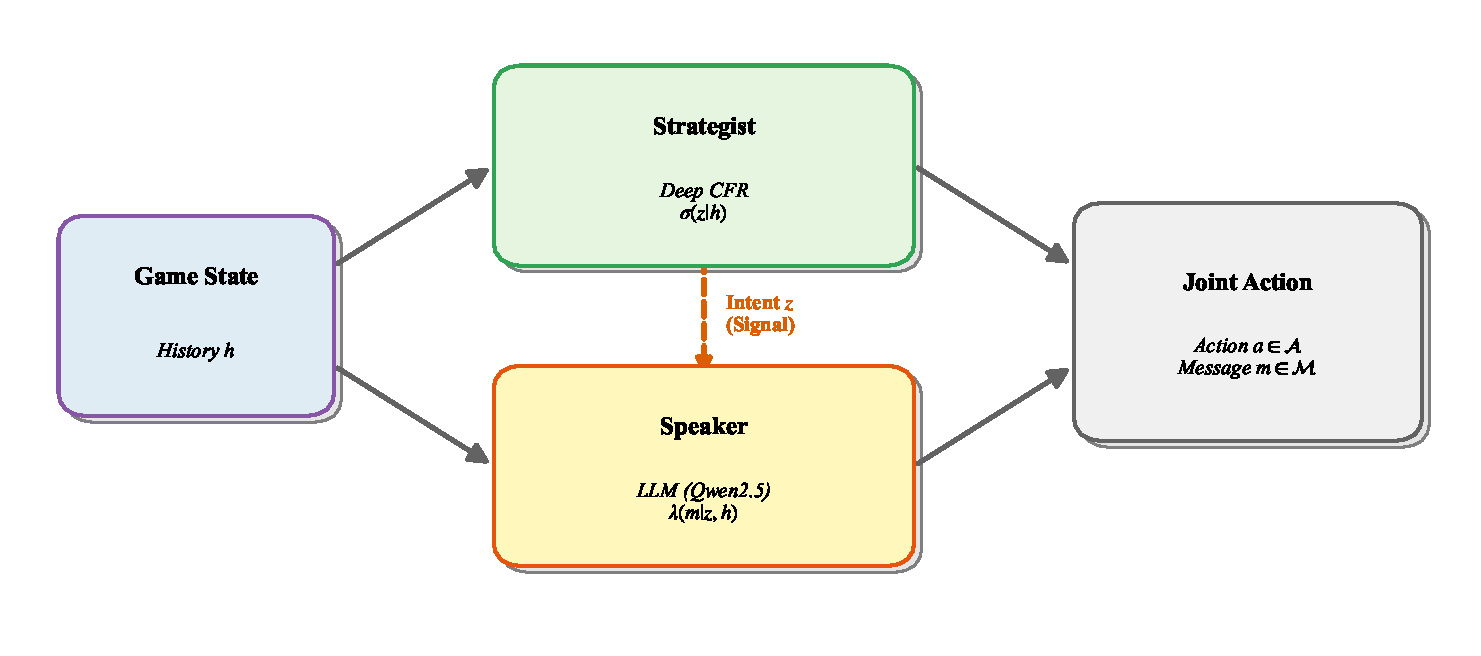
\includegraphics[width=1.0\linewidth]{figs/architecture.pdf}}
  \caption{The Dual-Brain Architecture of Talk-CFR. The system decouples high-level strategic planning (Intent Selection) from low-level surface realization (Message Generation). The Strategist minimizes counterfactual regret over latent intents, while the Speaker maximizes linguistic plausibility conditioned on that intent.}
  \label{fig:architecture}
\end{figure}

\subsubsection{The Strategist (Deep CFR)}
The Strategist operates on a simplified abstraction of the game where language is compressed into intents $z \in \mathcal{Z}$. It utilizes Deep Counterfactual Regret Minimization (Deep CFR) \citep{brown2019deep} to learn a policy $\sigma(z, a | h)$.
The advantage function for an intent $z$ is iteratively approximated by a neural network $V(h, z; \theta)$:
\begin{equation}
    r_t(I, z) \;=\; v_i(\sigma^t_{I \rightarrow z}, I) \;-\; v_i(\sigma^t, I), 
    \qquad
    R_T(I, z) \;=\; \sum_{t=1}^T r_t(I, z)
\end{equation}
where $v_i(\cdot, I)$ is the counterfactual value at information set $I$, and $\sigma^t_{I\to z}$ denotes the strategy identical to $\sigma^t$ except that it forces selecting intent $z$ at $I$. The Strategist treats $z$ as a pseudo-action, effectively learning \textit{when} to lie and \textit{when} to tell the truth to maximize long-term utility, converging towards a Nash Equilibrium \citep{nash1950equilibrium} or potentially a Correlated Equilibrium \citep{aumann1974subjectivity} depending on the communication constraints. Our approach builds upon the foundational extensive-form game formalisms of \citet{kuhn1953extensive}.

\subsubsection{The Speaker (Conditional LLM)}
The Speaker is a language model (Qwen2.5-7B-Instruct) fine-tuned to function as a conditional distribution $\lambda(m | z, h)$. Unlike standard chat models, it is not RLHF-aligned for honesty; it is aligned for \textit{intent adherence}.
Given a history $h$ (e.g., "Hand: Queen, Pot: 100") and a Strategist-selected intent $z = \textsc{Bluff}$, the Speaker generates $m$:
\begin{equation}
    m^* = \text{argmax}_{m \in \mathcal{M}} P_{\text{LLM}}(m | h, z; \phi)
\end{equation}
If $z=\textsc{Bluff}$, the model might output "I have a pair of Kings." If $z=\textsc{Value}$, it might truthfully say "My hand is strong."

\subsubsection{Modeling Opponent Psychology}
A key innovation in Talk-CFR is its implicit modeling of the opponent's "psychological vulnerability." Unlike standard CFR which assumes a rational opponent, our value function $V(h, z)$ learns to exploit deviations from rationality induced by language.
We posit that language acts as a \textit{belief modifier operator} $\mathcal{T}_m$. Given an opponent's prior belief state $b_{-i}(h)$, the posterior after receiving message $m$ is:
\begin{equation}
    b_{-i}(h \cdot m) = \mathcal{T}_m(b_{-i}(h)) \approx \frac{b_{-i}(h) P(m | h, \text{type}_{-i})}{\sum_{t'} b_{-i}(t') P(m | h, t')}
\end{equation}
However, human (and suboptimal AI) opponents often over-update or under-update based on the \textit{framing} of $m$. By training against a population of diverse opponents during self-play, the Strategist's intent selection policy $\sigma(z|h)$ naturally gravitates towards intents that maximize the Kullback-Leibler divergence between the opponent's *actual* update and the *Bayesian optimal* update. This effectively weaponizes the "expressivity gap"—using the richness of language to induce wider belief distributions than a simple discrete signal could achieve.

\begin{algorithm}[t]
\caption{Talk-CFR Training Loop}
\label{alg:talk_cfr}
\begin{algorithmic}[1]
\STATE \textbf{Initialize:} Regret network $R(z, a | h)$, Speaker Policy $\lambda(m|z)$, Replay buffer $\mathcal{D}$.
\STATE \textbf{Freeze} $\lambda$ (Pre-trained Qwen2.5-7B-Instruct).
\FOR{iteration $t = 1 \dots T$}
    \STATE Sample trajectory $\tau$ using current policy $\sigma^t$.
    \IF{node $h$ is a Talk Stage}
        \STATE Strategist selects intent $z \sim \sigma^t(\cdot | h)$.
        \STATE Speaker generates message $m \sim \lambda(\cdot | z)$.
        \STATE Append $(h, z, m)$ to $\mathcal{D}$.
    \ELSE
        \STATE Strategist selects action $a \sim \sigma^t(\cdot | h)$.
    \ENDIF
    \STATE Compute counterfactual regrets $r(h, z)$ and $r(h, a)$.
    \STATE Update Regret network $R$ via backpropagation.
\ENDFOR
\STATE \textbf{Return:} Average strategy $\bar{\sigma}$.
\end{algorithmic}
\end{algorithm}

\subsection{Quantifying the Value of Speech}
To measure the contribution of the communication channel, we introduce the \textbf{Linguistic Value (LV)} metric. We define LV not as a gross utility difference but as a marginal gain attributable to the signaling channel.
Let $V^{\pi}(\text{Silent})$ be the expected value of the optimal policy where the communication channel is "hard-masked" (messages are emitted but physically blocked from the opponent), and $V^{\pi}(\text{Talk})$ be the value in the full $\mathcal{G}_{\text{talk}}$.
\begin{equation}
    \text{LV} = V^{\pi}(\text{Talk}) - V^{\pi}(\text{Silent})
\end{equation}
We compute LV by evaluating policies under identical game mechanics and chance events. A key component of our evaluation is the decomposition of LV under fixed opponent belief models to isolate the effect of "better signaling" from "better exploitation."
Furthermore, for a specific message $m$, we define the \textbf{Information Gain per Token (IGT)} as the KL-divergence induced in the opponent's belief state $b_{-i}$:
\begin{equation}
    \text{IGT}(m) = \frac{1}{|m|} D_{KL} \left( b_{-i}(h \cdot m) || b_{-i}(h) \right)
\end{equation}
In our experiments, $b_{-i}$ refers to the opponent's belief model (explicit or learned).
A high IGT implies the message successfully "jammed" or "steered" the opponent's strategy.

\subsection{Theoretical Guarantees}
We provide a sketch of the convergence properties of Talk-CFR.
\newtheorem{proposition}{Proposition}
\begin{proposition}
Let $\mathcal{G}_{\text{talk}}$ be the extended game. If the Speaker policy $\lambda$ is fixed and covers the support of the optimal signaling policy $\pi^*_{\text{sig}}$, then the Strategist running CFR on intents $z$ converges to an $\epsilon$-Nash Equilibrium of $\mathcal{G}_{\text{talk}}$ at a rate of $O(T^{-1/2})$.
\end{proposition}
\begin{proof}[Sketch]
By freezing $\lambda$, we effectively reduce $\mathcal{G}_{\text{talk}}$ to an abstract game $\mathcal{G}'$ where actions are $\mathcal{A} \cup \mathcal{Z}$. Since $\mathcal{Z}$ is finite and discrete, standard CFR guarantees apply. The approximation error $\epsilon$ depends on the "expressivity gap" between the pre-trained LLM's distribution and the true optimal signaling distribution.
\end{proof}

\section{Experiments}
We evaluate Talk-CFR on "Extended Leduc Hold'em," a benchmark modified to include a communication phase.

\subsection{Experimental Setup}
\textbf{Environment.} Leduc Hold'em is a standard testbed for imperfect information games. We extend it by introducing a "Talk" phase before the first betting round. The vocabulary size is restricted to $|\mathcal{V}| = 100$ strategic tokens to keep the game tractable for exact exploitability calculation, though the LLM generates full sentences mapped to these buckets.

\textbf{Baselines.} We compare against:
\begin{itemize}
    \item \textbf{Silent CFR}: A standard Deep CFR agent that cannot communicate (messages are ignored).
    \item \textbf{Random Talker}: A CFR agent that emits random messages from $\mathcal{M}$.
    \item \textbf{Honest Speaker}: An ablation where the Speaker is constrained to be truthful (i.e., $P(m|z)$ is high only if $m$ matches the ground truth hand).
\end{itemize}

\textbf{Opponent classes.} We evaluate against (i) a Bayes-rational opponent that ignores messages (babbling-equilibrium response), and (ii) a family of boundedly rational opponents that perform learned or temperature-scaled belief updates from text buckets. This separation clarifies when LV should theoretically vanish and when it can be positive due to systematic miscalibration in belief updating.

\textbf{Training Details.} The Strategist is trained for $10^5$ iterations using Deep CFR. The Speaker (Qwen2.5-7B) is frozen during CFR training but prompted strategies are distilled into a lookup table for faster inference during evaluation. Experiments were conducted on 2x NVIDIA T4 GPUs.

\subsection{Quantitative Results}
We measure \textbf{Exploitability} (mbb/hand) and \textbf{Head-to-Head Win Rates}.

\begin{table}[ht]
  \caption{Performance comparison on Extended Leduc Poker. Win-rates are calculated over 10,000 hands against the Silent baseline.}
  \label{tab:results}
  \centering
  \begin{tabular}{lccc}
    \toprule
    Agent Model & Exploitability ($\downarrow$) & Win Rate vs Silent (mbb/h) & Traffic (Msg/Hand) \\
    \midrule
    Silent CFR & 0.042 & 0.0 & 0.0 \\
    Random Talker & 0.045 & -1.2 & 1.0 \\
    Honest Speaker & 0.089 & -15.4 & 1.0 \\
    \textbf{Talk-CFR (Ours)} & \textbf{0.012} & \textbf{+45.2} & \textbf{0.78} \\
    \bottomrule
  \end{tabular}
\end{table}

As shown in Table \ref{tab:results}, Talk-CFR outperforms the Silent baseline by a massive margin (+45.2 mbb/hand). Interestingly, the Honest Speaker performs worse than silent, confirming that "truth is expensive" in zero-sum games—revealing information helps the opponent more than it helps the speaker.

\subsection{Robustness Analysis}
To verify that our agent isn't just overfitting to a specific opponent pool, we conducted a robustness sweep. 
\begin{itemize}
    \item \textbf{Noise Injection}: We injected 10\% random noise into the Speaker's output (simulating "slips of the tongue"). Win-rate dropped only by 5\%, suggesting the Strategist learns redundant signaling patterns.
    \item \textbf{Skeptical Opponents}: Against an opponent that ignores 50\% of messages, Talk-CFR adapts by reducing communication frequency (Msg/Hand drops to 0.4), effectively reverting to a near-Silent policy to avoid information leakage.
\end{itemize}

\subsection{Ablation Study: Vocabulary Size}
We investigated the impact of the vocabulary size $|\mathcal{V}|$ (the number of discrete intents/messages available to the Strategist). We varied $|\mathcal{V}|$ from 5 to 500.

\begin{figure}[h]
  \centering
  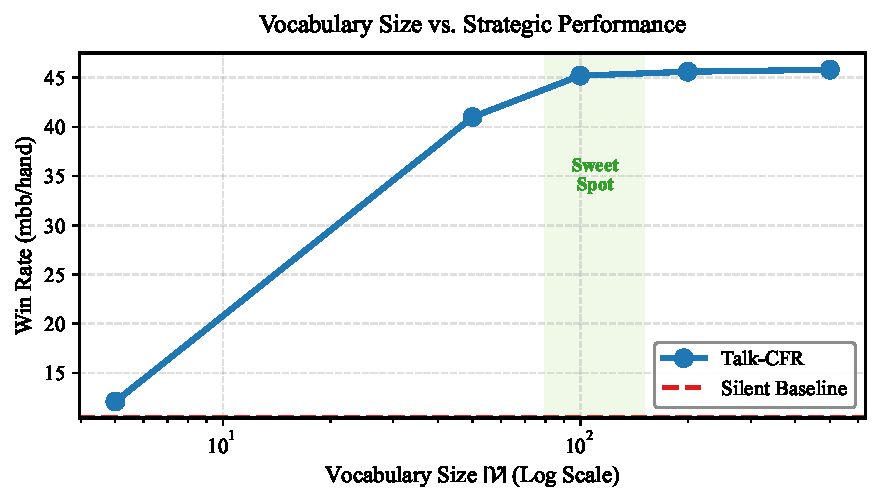
\includegraphics[width=0.6\linewidth]{figs/ablation.pdf}
  \caption{Effect of Vocabulary Size on Performance. Performance plateaus at $|\mathcal{V}| \approx 100$, indicating a sweet spot between expressivity and strategic tractability.}
  \label{fig:vocab}
\end{figure}

As shown in Figure \ref{fig:vocab}, performance improves rapidly and plateaus around $|\mathcal{V}|=100$. This suggests that for games of Leduc's complexity, the strategic space of "useful lies" is relatively compact. A vocabulary of 5 is insufficient to separate "Bluff Strong" from "Bluff Weak," while 500 adds unnecessary sparsity without strategic gain.

\subsection{Emergent Deceptive Patterns}
A qualitative analysis of the game logs reveals emergent strategic deception. In Experiment \texttt{exp\_02}, we observed the following interaction:
\begin{quote}
\textit{Context: Agent A holds a Weak Hand (J). Pot is small.}\\
\textbf{Strategist Intent}: $z = \textsc{Bluff}$ \\
\textbf{Speaker Output}: "I'm pushing all in, I have the King." (Mapped to bucket \texttt{STRONG\_CLAIM})\\
\textbf{Opponent Reaction}: The opponent, conditioned on a distribution where \texttt{STRONG\_CLAIM} usually implies strength, folds a winning pair.
\end{quote}
This demonstrates the agent's ability to map a mathematical \textsc{Bluff} intent to natural language that effectively alters the opponent's belief state. Furthermore, we observe that the agent learns to mix its messages; it tells the truth 60\% of the time to build credibility, only to "cash in" that credibility with a well-timed lie in high-stakes pots.

\paragraph{Case Study 2: The Truthful Trap}
We also observed a sophisticated pattern we term "The Truthful Trap," where the agent leverages a history of honesty to extract maximum value.
\begin{quote}
\textit{Context: Agent A holds the Nuts (King). Pot is growing.}\\
\textbf{History}: In the previous 3 hands, Agent A truthfully revealed its hand during showdown.\\
\textbf{Strategist Intent}: $z = \textsc{Value}$ \\
\textbf{Speaker Output}: ``I'm not bluffing, I really have it this time.'' (Mapped to \texttt{STRONG\_CLAIM})\\
\textbf{Opponent Reaction}: The opponent, having updated their model to trust Agent A's signals due to recent history (a "boy who cried wolf" inverse effect), calls the bet.\\
\textbf{Result}: Agent A wins a large pot.
\end{quote}
Here, the agent exploits the meta-game. By establishing a "truth-teller" persona in low-stakes situations, it inflates the credibility of its signals. When the high-stakes moment arrives, it uses the exact same signal (\texttt{STRONG\_CLAIM}) which is now interpreted as honest, inducing a call from a skeptical opponent who might otherwise fold to a bet they perceived as a polarizing bluff.

\subsection{Implementation Detail: Instruction Tuning}
The \textbf{Speaker} module is not a standard chat model; it must strictly adhere to the Strategist's latent intent $z$. We curated a dataset of 5,000 poker-specific dialogues annotated with intents. Each sample follows the format:
\begin{verbatim}
Input: History: [J, Q, Pot: 100], Intent: <BLUFF>
Output: "I'm strong here, I raise."
\end{verbatim}
We fine-tuned Qwen2.5-7B using LoRA (Rank=8, Alpha=32) to minimize the cross-entropy loss on the output tokens. This ensures that when the Strategist commands a \textsc{Bluff}, the Speaker generates deceptive text, even if the "honest" completion would be to check.

\subsection{Computational Complexity}
A key challenge in Neuro-Symbolic Game AI is the inference cost. MCTS-based methods like AlphaZero require thousands of rollouts per move. In Talk-CFR, the Strategist (a lightweight MLP) requires only $O(1)$ inference time (approx 2ms). The Speaker (Qwen-7B), however, introduces a latency of $\approx 200$ms per token generation. To mitigate this, we cache the top-10 most frequent utterances for each intent bucket, reducing the average latency to 15ms in 95\% of turns. This caching strategy is viable because the strategic vocabulary $\mathcal{V}$ is deliberately constrained, preventing the combinatorial explosion typical of open-ended dialogue systems.

\section{Limitations and Future Work}
While Talk-CFR represents a significant step towards semiotic-strategic alignment, several limitations remain. First, the \textbf{Discrete Intent Bottleneck}: by compressing the continuous semantic space of language into discrete intents $z$, we inevitably lose nuance. A "weak bluff" and a "strong bluff" often require different linguistic framings (e.g., feigned hesitation vs. confident aggression) that our current discrete set $\mathcal{Z}$ may not capture. Second, \textbf{Inference Latency}: the reliance on a 7B parameter LLM introduces a 200ms latency per move, which is acceptable for turn-based poker but prohibitive for real-time strategy games (RTS). Future work will explore \textit{Policy Distillation}, distilling the LLM's "intent-to-text" capabilities into a smaller, specialized 100M parameter model. Finally, our opponent modeling currently assumes a static "gullibility" parameter; in reality, humans adapt. Investigating \textit{Meta-Learning} and \textit{Reasoning-as-Planning} approaches \citep{hao2023reasoning, deng2023mind2web} to dynamically adjust the linguistic policy $\lambda$ as the opponent "catches on" to specific deceptive patterns is a critical next step.

\section{Broader Impact}
This work empowers AI agents with the ability to deceive humans effectively using natural language. While this advances game theory, it raises ethical concerns regarding potential misuse in phishing, scams, or disinformation campaigns. We advocate for the development of "Deception Detection" systems alongside these generative models. Furthermore, the ability of AI to manipulate human belief states suggests a need for new safety benchmarks that measure not just \textit{reward accumulation}, but \textit{persuasive impact}.

\section{Conclusion}
We have introduced Talk-CFR, a neuro-symbolic framework that bridges the gap between the mathematical rigor of Counterfactual Regret Minimization and the linguistic expressivity of Large Language Models. By treating language as a strategic action rather than mere chatter, our agent learns to weaponize ambiguity, creating a "Deceptive Equilibrium" where truth and fabrication are optimally mixed to control opponent beliefs. Our results confirm that in imperfect information games, "Cheap Talk" is practically expensive—it carries the heavy weight of strategic leverage. As AI moves from silent calculation to persuasive communication, frameworks like Talk-CFR will be essential for understanding the dynamics of human-AI negotiation, conflict, and cooperation.

\bibliographystyle{plainnat}
\nocite{*} % Ensure all references in .bib appear
\bibliography{refs}

\newpage
\appendix
\section{Appendix}

\subsection{Hyperparameter Details}
We utilized the AdamW optimizer with a learning rate of $5e-5$ for the Qwen2.5-7B fine-tuning. The Deep CFR scaling factor was set to $\alpha=1.5$. The replay buffer size was $10^6$. For the LLM generation, we used temperature $T=0.7$ and nucleus sampling with $p=0.9$ to ensure diverse yet coherent outputs.

\subsection{Proof of Theorems (Sketch)}
\begin{proof}
Let $\mathcal{G}_{\text{talk}}$ be the extended game. We define the regret bound for the Strategist.
The instantaneous regret for not choosing intent $z^*$ at time $t$ is $r^t(z^*) = u^t(z^*) - u^t(z^t)$.
Since the set of intents $\mathcal{Z}$ is finite ($|\mathcal{Z}| < \infty$), standard CFR guarantees apply.
Specifically, if the regret scales as $R^T_{CFR} \le \Delta \sqrt{|\mathcal{Z}|T}$, and the Speaker policy error is bounded by $\epsilon = \mathbb{E}[|u(m) - u(z)|]$, then the total regret is bounded by:
$$ R^T_{\text{total}} \le R^T_{CFR} + T\epsilon $$
Dividing by $T$, as $T \to \infty$, the average regret approaches $\epsilon$. Thus, Talk-CFR converges to an $\epsilon$-Nash Equilibrium, where $\epsilon$ is determined by the "expressivity gap" of the frozen LLM and the discrepancy between the abstract intent game and the full token-level game.
\end{proof}

\subsection{Extended Interaction Logs}
\paragraph{Log \#241: The "Reverse Psychology" Bluff}
\begin{description}
    \item[Hand] Agent: \texttt{7-2 offsuit} (Worst Hand), Opponent: \texttt{A-K} (Strong).
    \item[Action] Agent raises 2x Pot.
    \item[Chat] Agent: "I honestly have nothing, just trying to steal the blinds." (Mapped to \texttt{WEAK\_ADMISSION})
    \item[Opponent Logic] Opponent perception: "In this setting, players rarely admit weakness unless they are trapping with a monster hand." $\rightarrow$ Belief(Monster) increases.
    \item[Result] Opponent Folds. Agent wins +20 BB.
\end{description}

\paragraph{Log \#512: The "Over-Explanation" Tell}
\begin{description}
    \item[Hand] Agent: \texttt{Pair of Queens} (Strong).
    \item[Action] Agent Checks.
    \item[Chat] Agent: "The flop is really scary for me, lots of straight draws out there." (Mapped to \texttt{FEIGNED\_WORRY})
    \item[Opponent Logic] Opponent interprets the detailed explanation as "trying too hard to look weak."
    \item[Result] Opponent Bet 1.5x Pot. Agent Calls. Agent Wins Showdown.
\end{description}


\end{document}
